\documentclass[12pt]{article}

\usepackage{booktabs}% http://ctan.org/pkg/booktabs
\usepackage[utf8]{inputenc}
\usepackage{changepage}
\usepackage{pgfplots}
\usepackage{amssymb}
\usepackage{xcolor}
\usepackage{hyperref}
\usepackage{listings}
\usepackage[T1]{fontenc}
\usepackage[utf8]{inputenc}
\usepackage{adjustbox}
\usepackage{amsmath}
\usepackage{mathtools}
\usepackage{biblatex}
\lstset{
  language=Python,
  numbers=left,
  numberstyle=\tiny,
  stepnumber=1,
  numbersep=5pt,
  tabsize=4,
  basicstyle=\ttfamily,
  columns=fullflexible,
  keepspaces,
}
\hypersetup{
    colorlinks,
    citecolor=black,
    filecolor=black,
    linkcolor=black,
    urlcolor=black
}

% Set page size and margins
% Replace `letterpaper' with `a4paper' for UK/EU standard size
\usepackage[letterpaper,top=2cm,bottom=2cm,left=3cm,right=3cm,marginparwidth=1.75cm]{geometry}

% Useful packages
\usepackage{amsmath}
\usepackage{mathtools}
\usepackage{graphicx}
\newenvironment{para}{\begin{adjustwidth}{13mm}{}}{\end{adjustwidth}}

\newcommand\tab[1][1cm]{\hspace*{#1}}

\newcommand{\tabitem}{\llap{\textbullet}}
\newcommand{\Hsquare}{%
\text{\fboxsep=-.2pt\fbox{\rule{0pt}{1ex}\rule{1ex}{0pt}}}%
}

\newtheorem{Definizione}{Definizione}[subsection]
\newtheorem{Lemma}{Lemma}[subsection]
\newtheorem{Teorema/Definizione}{Teorema/Definizione}[subsection]
\newtheorem{Corollario}{Corollario}[subsection]
\newtheorem{Teorema}{Teorema}[subsection]
\newtheorem{Proposizione}{Proposizione}[subsection]
\newtheorem{Notazione}{Notazione}[subsection]
\newtheorem{Commento}{Commento}[subsection]
\newtheorem{Dimostrazione}{Dimostrazione}[subsection]
\newtheorem{Osservazione}{Osservazione}[subsection]
\newtheorem{Nota}{Nota}[subsection]

\title{RSO: Sistemi Operativi}
\author{spitfire}
\date{A.A. 2023-2024}
\begin{document}
\begin{figure}
    \centering
    
\includegraphics[width=0.35\textwidth]{Images/Logo scienze bicocca.png}
\end{figure}

\vspace{10cm}
\date{A.A. 2023-2024}


\maketitle

\newpage

\tableofcontents
\newpage

\section{Struttura e servizi}
Cosa sappiamo sui sistemi operativi? Sappiamo che, per esempio, i principali sono
\textbf{linux, Windows e MacOS}; che il sistema operativo è il 
\textbf{primo programma che viene eseguito dopo il boot}. Di solito un sistema operativo
fornisce un \textbf{ambiente desktop a finestre e ci permette di installare nuove applicazioni}.
Ci permette inoltre di eseguire tante applicazioni \textbf{contemporaneamente}, anche più dei \textbf{core dei processori}.
Inoltre, esso \textbf{mantiene e organizza i nostri dati sotto forma di file e cartelle}.
Quindi, cos'è un \textbf{sistema operativo}? Esso è:
\begin{itemize}
    \item Un insieme di \textbf{programmi} (Software)
    \item Che gestiscono \textbf{gli elementi fisici di un computer} (Hardware)
\end{itemize}
E a \textbf{cosa serve un sistema operativo}?
\begin{itemize}
    \item Fornire una \textbf{piattaforma di sviluppo per le applicazioni}, che permette loro di \textbf{condividere e astrarre} le risorse HW.
    \item Agisce da \textbf{intermediario} tra utenti e computer, permettendo agli utenti di \textbf{controllare l'esecuzione dei programmi applicativi} e l'assegnazione delle risorse HW ad essi
    \item \textbf{Protegge le risorse degli utenti} (e dei loro programmi) dagli altri utenti (e dai loro programmi) e da eventuali \textbf{attori esterni}
\end{itemize}
Un sistema operativo è quindi in primo luogo una \textbf{piattaforma di sviluppo}, ossia un insieme di funzionalità software che i programmi applicativi possono usare.
Tali funzionalità permettono ai programmi di poter usare in maniere conveniente le risorse hardware di condividerle:
\begin{itemize}
    \item Da un lato il sistema operativo \textbf{astrae} le risorse hardware, presentando agli sviluppatori di programmi applicativi una visione delle risorse hardware più facile da usare e più potente rispetto alle risorse hardware "native".
    \item Dall'altro, il sistema operativo \textbf{condivide} le risorse hardware tra molti programmi contemporaneamente in esecuzione, suddividendole tra i programmi in maniera equa ed efficiente e controllando che questi le usino correttamente.
\end{itemize}
\subsection{Componenti di un sistema di elaborazione}
Le componenti di un sistemi di elaborazione sono:
\begin{itemize}
    \item \textbf{Utenti}: Persone, macchine, altri computer, ecc...
    \item \textbf{Programmi applicativi}: Risolvono i problemi di calcolo degli utenti
    \item \textbf{Sistema operativo}: Coordina e controlla l'uso delle risorse hardware
    \item \textbf{Hardware}: Risorse di calcolo (CPU, periferiche, memoria di massa, ...)
\end{itemize}
\begin{center}
    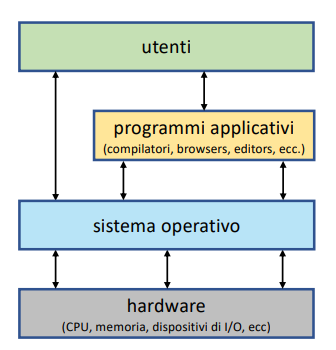
\includegraphics[width = 0.50\textwidth]{Images/1.PNG}
\end{center}
\subsection{Requisiti per i sistemi operativi}
Oggigiorno i computer sono ovunque: vi sono molteplici tipologie di computer utilizzati in scenari
applicativi molto diversi. In quasi tutti i tipi di computer si tende ad installare un sistema operativo allo scopo
di gestire l'hardware e semplificare la programmazione. Ma ogni scenario applicativo in cui viene usato un computer
richiede che il sistema operativo che vi viene installato abbia caratteristiche ben determinate. Che cosa si richiede quindi
ad un sistema operativo per supportare uno determinato scenario applicativo?
Vediamo qualche scenario:
\begin{itemize}
    \item \textbf{Server e Mainframe}: massimizzare le performance, rendere equa la condivisione delle risorse tra molti utenti
    \item \textbf{Laptop, PC e tablet}: massimizzare la facilità d'uso e la produttività della singola persona che lo usa
    \item \textbf{Dispositivi mobili}: Ottimizzare i consumi energetici e la connettività
    \item \textbf{Sistemi embedded}: funzionare senza, o con minimo, intervento umano e reagire in tempo reale agli stimoli esterni (interrupt)
\end{itemize}
\subsection{La maledizione della generalità}
Nella storia (ed anche oggi) alcuni sistemi operativi sono stati utilizzati per scenari applicativi diversi.
Ad esempio, Linux è usato oggi nei server, nei computer desktop e nei dispositivi mobili (come parte di Android).
La \textbf{maledizione della generalità} afferma che, se un sistema operativo deve supportare un insieme di scenari applicativi troppo ampio,
non sarà in grado di supportarne nessuno particolarmente bene. Esempio di questo si è visto con \textbf{OS/360}, il primo sistema operativo che doveva supportare
una famiglia di computer diversi (la linea 360 IBM).
\subsection{Struttura dei sistemi operativi}
Non c'è una definizione universalmente accettata di quali programmi fanno pare di un sistema operativo. In generale però un sistema operativo almeno comprende:
\begin{itemize}
    \item \textbf{Kernel}: Il "programma sempre presente" che si "impadronisce" dell'HW, lo gestisce, ed offre ai programmi i servizi per poterlo usare in maniera condivisa ed astratta
    \item \textbf{Middleware}: servizi di alto livello che astraggono ulteriormente i servizi del kernel e semplificano la programmazione di applicazioni (API, framework per grafica e per suono,...)
    \item \textbf{Programmi di sistema}: Non sempre in esecuzione, offrono ulteriori funzionalità di supporto e di interazione utente con il sistema (gestione di processi e jobs, UI, ...)
\end{itemize}
Alcuni sistemi operativi forniscono "out-of-the-box" anche dei \textbf{programmi applicativi} (editor, fogli di calcolo,...) ma non li considereremo come parti del sistema operativo.
Data questa lista di componenti, possiamo rivisitare le \textbf{componenti di un sistema di elaborazione}:
\begin{center}
    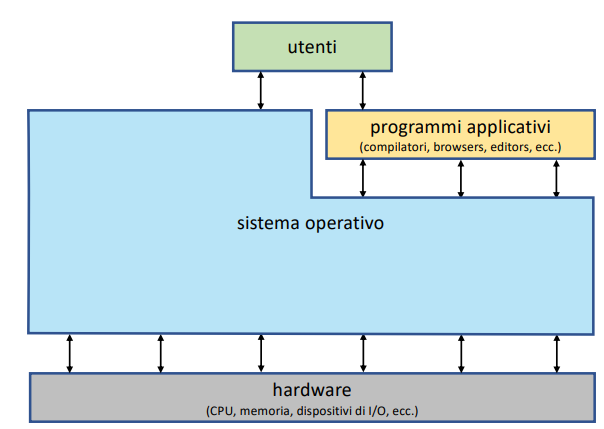
\includegraphics[width = 0.55\textwidth]{Images/2.PNG}
\end{center}
Che visti in dettaglio diventano:
\begin{center}
    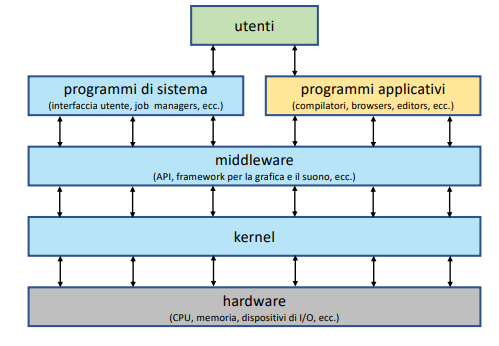
\includegraphics[width = 0.63\textwidth]{Images/3.PNG}
\end{center}
\subsection{Servizi offerti da un sistema operativo}
I principali servizi che un sistema operativo offre sono:
\begin{itemize}
    \item \textbf{Controllo processi}: questi servizi permettono di caricare in memoria un programma, eseguirlo, identificare la sua terminazione e registrarne la condizione di terminazione (normale o erronea)
    \item \textbf{Gestione dei file}: questi servizi permettono di leggere, scrivere e manipolare files e directories
    \item \textbf{Gestione dispositivi}: questi servizi permettono ai programmi di effettuare operazioni di input/output, ad esempio leggere da/scrivere su un terminale
    \item \textbf{Comunicazione interprocesso}: i programmi in esecuzione possono collaborare tra di loro scambiandosi informazioni: questi servizi permettono ai programmi in esecuzione di comunicare
    \item \textbf{Protezione e sicurezza}: permette ai proprietari delle informazioni in un sistema multiutente o in rete di controllarne l'uso da parte di altri utenti e di difendere il sistema dagli accessi illegali
    \item \textbf{Allocazione delle risorse}: alloca le risorse hardware (CPU, memoria, dispositivi di I/O) ai programmi in esecuzione in maniera equa ed efficiente
    \item \textbf{Rilevamento errori}: gli errori possono avvenire nell'hardware o nel software  (es. divisione per 0); quando avvengono il sistema operativo deve intraprendere opportune azioni (recupero, terminazione del programma o segnalazione della condizione di errore al programma)
    \item \textbf{Logging}: mantiene traccia di quali programmi usano quali risorse, allo scopo di contabilizzarle
\end{itemize}
\subsection{Chiamate di sistema e Application Programming Interfaces}
\begin{center}
    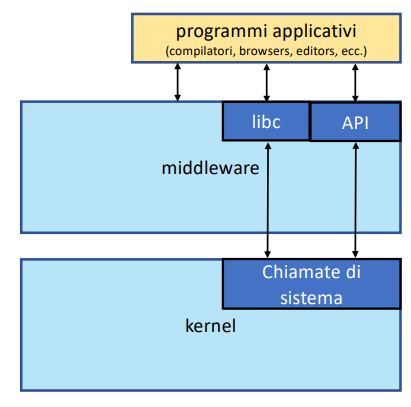
\includegraphics[width = 0.50\textwidth]{Images/4.PNG}
\end{center}
Il kernel offre i propri servizi ai programmi come \textbf{chiamate di sistema} (syscalls), ossia funzioni invocabili in un determinato linguaggio di programmazione (C, C++, ...).
I programmi però non utilizzano direttamente le chiamate di sistema, ma delle librerie di middleware dette \textbf{Application Programming Interface} (API) implementate invocando le chiamate di sistema.
Spesso le API sono fortemente legate con le librerie standard del linguaggio di implementazione (es. libc se le API sono implementate in C) al punto che anche queste diventano parte implicita dell'API.
Bisogna ricordare che:
\begin{itemize}
    \item Le API sono \textbf{esposte dal middleware}, mentre le chiamate di sistema \textbf{dal kernel}
    \item Le API usano le chiamate di sistema nella loro implementazione
    \item Le API sono standardizzate (es. POSIX, Win32), le chiamate di sistema no, quindi ogni kernel ha chiamate di sistema differenti
    \item Le API sono stabili, le chiamate di sistema possono variare al variare della versione del sistema operativo
    \item Le API offrono funzionalità più ad alto livello e più semplici da usare, le chiamate di sistema offrono funzionalità più elementari e più complesse da usare
\end{itemize}
\begin{center}
    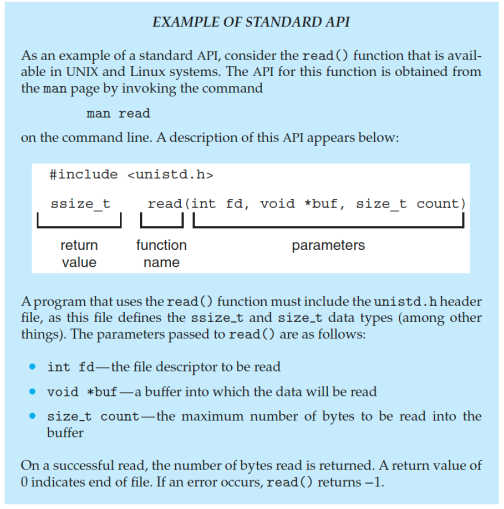
\includegraphics[width = 0.75\textwidth]{Images/5.PNG}
\end{center}
\subsection{Programmi di sistema}
La maggior parte degli utenti utilizza servizi del sistema operativo attraverso i programmi di sistema.
Questi permettono agli utenti di avere un ambiente più conveniente per l'esecuzione dei programmi, il loro sviluppo e la gestione delle risorse del sistema.
Vi sono diversi tipi di programmi di sistema:
\begin{itemize}
    \item \textbf{Interfacce utente (UI)}: permette agli utenti di interagire con il sistema stesso; può essere grafica (GUI) o a riga di comando (CLI); i sistemi mobili hanno un'interfaccia touch.
    \item \textbf{Gestione file}: creazione, modifica e cancellazione di file e directories
    \item \textbf{Modifica dei file}: editor di testo, programmi per la manipolazione del contenuto dei file (Emacs)
    \item \textbf{Visualizzazione e modifica informazioni di stato}: data, ora, memoria disponibile, processi, utenti, ... fino a informazioni complesse su prestazione, accessi al sistema e debug. Alcuni sistemi implementano un \textbf{registry}, ossia un database delle informazioni di configurazione
    \item \textbf{Caricamento ed esecuzione dei programmi}: loader assoluti e rilocabili, linker e debugger
    \item \textbf{Ambienti di supporto alla programmazione}: compilatori, assemblatori, debugger, interpreti per diversi linguaggi di programmazione
    \item \textbf{Comunicazione}: forniscono i meccanismi per creare connessione tra utenti, programmi e sistemi; permettono di inviare messaggi agli schermi di un altro utente, di navigare il web, di inviare messaggi di posta elettronica, di accedere remotamente ad un altro computer, di trasferire i file, ecc...
    \item \textbf{Servizi di background}: lanciati all'avvio, alcuni terminano, altri continuano l'esecuzione fino allo shutdown. Forniscono servizi quali verifica dello stato dei dischi, scheduling di jobs, logging, ...
\end{itemize}
\subsubsection{Intefaccia utente: l'interpete dei comandi}
\begin{center}
    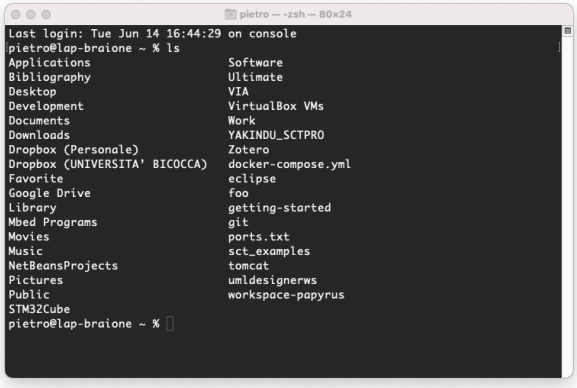
\includegraphics[width = 0.75\textwidth]{Images/6.PNG}
\end{center}
L'interprete dei comandi permette agli utenti di impartire in maniera testuale delle istruzioni al sistema operativo.
In molti sistemi operativi è possibile configurare quale interprete dei comandi usare, nel qual caso è detto \textbf{shell}.
Ci sono due modi per implementare un comando:
\begin{itemize}
    \item \textbf{Built-in}: l'interprete esegue direttamente il comando (tipico dell'interprete dei comandi di Windows)
    \item \textbf{Come programma di sistema}: l'interprete manda in esecuzione un programma (tipico delle shell Unix e Unix-Like)
\end{itemize}
Spesso l'interprete riconosce \textbf{un vero e proprio linguaggio di programmazione} (es. Bash).
\subsubsection{Interfaccia utente: le interfacce grafiche}
\begin{center}
    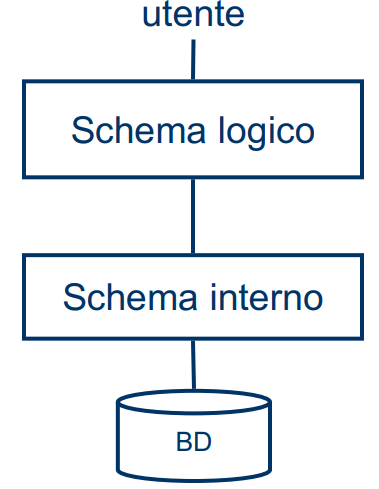
\includegraphics[width = 0.85\textwidth]{Images/7.PNG}
\end{center}
Le interfacce grafiche(GUI) sono di solito basate sulla metafora della scrivania, delle icone e delle cartelle (corrispondenti alle directory).
Nate dalla ricerca presso lo Xerox PARC lab negli anni 70, vennero popolarizzate dai computer Apple Macintosh negli anni 80. Su Linux le più popolari sono KDE e Gnome.
\newpage
\subsubsection{Intefaccia utente: Le interfacce touch-screen}
\begin{center}
    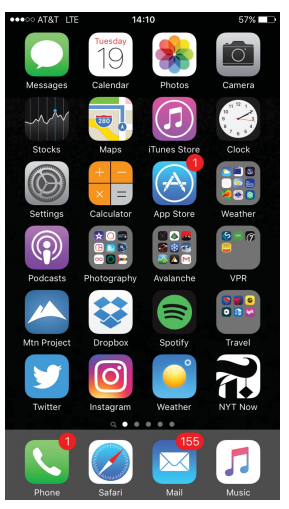
\includegraphics[width = 0.30\textwidth]{Images/8.PNG}
\end{center}
I dispositivi mobili richiedono interfacce di nuovo tipo. Esse non prevedono nessun dispositivo di puntamento (mouse); sostituendolo con l'uso dei gesti (gestures).
Inoltre esse possono offrire servizi come tastiere virtuali e comandi vocali.
\subsection{L'implementazione dei programmi di sistema}
\begin{center}
    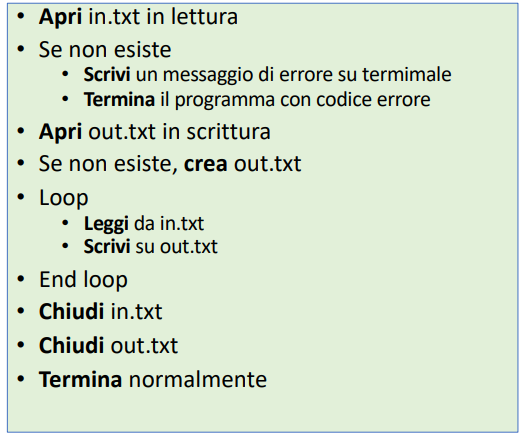
\includegraphics[width = 0.55\textwidth]{Images/9.PNG}
\end{center}
I programmi di sistema sono implementati utilizzando le API, esattamente come i programmi applicativi.
Consideriamo ad esempio il comando \textit{cp} delle shell dei sistemi operativi Unix-like; la sua sintassi è:
\begin{center}
    \textit{cp in.txt out.txt}
\end{center}
Esso copia il contenuto del file \textit{in.txt} in un file \textit{out.txt}. Se il file \textit{out.txt} esiste, il contenuto precedente viene cancellato, altrimenti \textit{out.txt} viene creato.
L'immagine sopra rappresenta una possibile struttura del codice; le invocazioni delle API sono riportate in grassetto.
\textit{cp} è implementato come programma di sistema.
\section{Processi e thread: i servizi}
Un sistema operativo esegue un certo numero di programmi sullo stesso sistema di elaborazione.
Il numero di programmi da eseguire può essere arbitrariamente elevato, di solito è infatti molto maggiore del numero di CPU del sistema.
A tale scopo, il sistema operativo realizza e mette a disposizione un'astrazione detta \textbf{processo}. Un processo è quindi un'entità attiva astratta definita dal sistema operativo allo scopo di eseguire un programma.
Per il momento, assumiamo che l'esecuzione di un processo sia sequenziale, tuttavia \textbf{rilasseremo presto questa assunzione}.
\subsection{Programmi e processi}
È fondamentale notare la differenza tra programma e processo!
\begin{itemize}
    \item Un programma è un'entità passiva (un insieme di istruzioni, tipicamente contenuto in un file sorgente o eseguibile)
    \item Un processo è un'entità attiva (è un \textbf{esecutore di un programma} o un \textbf{programma in esecuzione})
\end{itemize}
Uno stesso programma può dare origine a \textbf{diversi processi}:
\begin{itemize}
    \item Diversi utenti eseguono lo stesso programma
    \item Uno stesso programma viene eseguito più volte, anche contemporaneamente, dallo stesso utente
\end{itemize}
\subsection{Struttura di un processo}
Un processo è composto da diverse parti:
\begin{itemize}
    \item 
\end{itemize}
\end{document}